\chapter{Perception: Individual variability in the decoding of multiple prosodic and non-prosodic cues to prominence}
\label{ch: Perception}
\chaptermark{Perception study}

\section{Overview}

This chapter presents the findings of a perception study to complement the two production studies discussed in the preceding chapters. We conducted a prominence rating task on visual analogue scales to probe the effects of multiple prosodic (categorical and continuous), syntactic, and semantic-pragmatic cues on the perception of prominence in German listeners. Recordings collected as part of the study presented in Chapter \ref{ch:Production II} were used as stimuli. At the individual level, we will explore how and to what extent listeners differ in their response to these different prominence cues.

Prominence perception is influenced by a variety of factors related to several linguistic levels (see Chapter \ref{ch:background prominence}). Beside prosody, lexical factors (e.g., word frequency and part-of-speech) have been found to play a role for the perception of prominence in German in previous studies \citep[e.g.,][]{baumannWhatMakesWord2018, wagnerExploitingSpeechgestureLink2019}. What is more, listeners may respond to different cues in their decoding of prominence. For example, \citet{baumannWhatMakesWord2018} found that some listeners paid more attention to prosodic variables, especially those related to the F0 contour, while other listeners relied more on lexical and semantic-syntactic factors, such as lexical frequency, part-of-speech, and the presence or absence of a focus particle. Similarly, \citet{wagnerExploitingSpeechgestureLink2019} observed that some listeners relied more on prosodic cues, such as duration, intensity, and F0 changes, and others more on structural cues, e.g., part-of-speech and stressability, in their prominence perception. \citet{orricoInfluenceEmpathyAutisticlike2023}, testing the effects of accent type (H* versus L+H*) and contrastiveness on the perception of prominence in British English participants, found some listeners to be guided more by phonetics (i.e., accent type) and others by pragmatics (i.e., contrastiveness). However, these studies did not consider discourse context, only presenting isolated sentences in their prominence rating tasks. We plan on expanding on this line of research by considering multiple prosodic and non-prosodic variables in a prominence rating task. By presenting stimuli in context, we are able to consider nuanced discourse meaning in the form of lexical and referential information status. A similar study has previously been conducted by \citet{coleSignalbasedExpectationbasedFactors2010}, who presented longer stretches of speech in an RPT task in American English and investigated repetition as a potential predictor of prominence, among other cues. Nevertheless, our approach to discourse meaning is more differentiated and our main objective is to investigate individual differences in the effects of these factors on the perception of prominence. In addition, we consider syntactic factors, i.e., grammatical role and position in the sentence, which adds another linguistic layer that has previously received less attention in prominence perception studies. Syntactic structure is known to interact with prosodic structure (see Section \ref{section: lexical and syntactic}) and it has been shown that individual speakers differ in their mapping of the two domains \citep{huttenlauchIndividualVariabilityProsodic2022}. Considering these two classes of non-prosodic factors in addition to several categorical and continuous prosodic variables will thus lend new insights with regard to individual listener preferences or similarities in the perception of prominence.

In the weighting of these variables, we expect categorical prosodic cues, such as accent status and accent type, to play a particularly important role for prominence perception as previous studies on West-Germanic languages have already demonstrated \citep[e.g.,][]{baumannWhatMakesWord2018, wagnerExploitingSpeechgestureLink2019, bishopPhonologyPhoneticsSignalextrinsic2020}. However, listeners may differ in their weighting of the available cues, some potentially being driven more by prosodic and others by non-prosodic cues. As in the previously presented production study (see Chapter \ref{ch:Production II}), we collected information on participants' communicative skill as a possible explanation for such differences in behavior. In line with prior observations \citep[e.g.,][]{bishopPhonologyPhoneticsSignalextrinsic2020, orricoInfluenceEmpathyAutisticlike2023}, we expect listeners with higher communicative skill to be more sensitive to prosodic prominence cues. 

The results of the present study confirm that most prosodic parameters affect prominence ratings in an expectable way: Higher values in the continuous prosodic parameters generally result in higher prominence ratings, words with a nuclear accent are perceived as more prominent than prenuclear accented and deaccented words and the hierarchy of perceived prominence of pitch accent types largely confirms previous findings \citep[e.g.,][]{baumannPerceptualProminencePitch2015}. Among the prosodic variables, accent status, word duration, and accent type are the most important predictors of prominence, while the non-prosodic cues play only a subordinate role. Across listeners, there are only subtle differences in the sensitivity to and weighting of cues. One group of listeners is more strongly affected by all cues, prosodic and non-prosodic, in their prominence ratings, weighting accent status and accent type most highly, while the other group is less sensitive to all cues and guided most strongly by accent status and word duration. Evidence for an effect of communicative skill is weak.

The remainder of this chapter is structured as follows: In Section \ref{sec:s3_methods}, we describe the stimuli, data collection procedure, and participants as well as the statistical methods used in the analysis. Section \ref{sec:s3_results} presents the results of the study starting with an overview of the overall results across participants before narrowing in on individual differences and similarities in the observed patterns. Finally, Section \ref{sec:s3_discussion} concludes with an interim discussion of this chapter's findings.

\section{Methods} \label{sec:s3_methods}

\subsection{Stimuli, procedure, and participants}

We conducted a prominence rating task with gradual visual analogue scales (or slider scales) ranging from 0 to 100 implemented online in SoSci Survey \citep{leinerSoSciSurvey2024}. Participants were presented with 47 short excerpts of written text and corresponding audio consisting of three to five sentences. They were asked to rate how highlighted an underlined target word sounded to them after listening to the whole excerpt (see Figure \ref{fig:S3_soscisurvey} for a screenshot of an example task). Participants were allowed to listen to the excerpts as many times as they liked. The 47 target items were preceded and followed by five items sampled from different stories, which did not enter the analysis, to serve as practice items and to counteract potential effects of declining attention. After the completion of the prominence rating task, participants were asked to provide basic sociodemographic information and fill out a short questionnaire on their communicative skill. The whole procedure took on average 20 minutes.

\begin{figure}[t]
		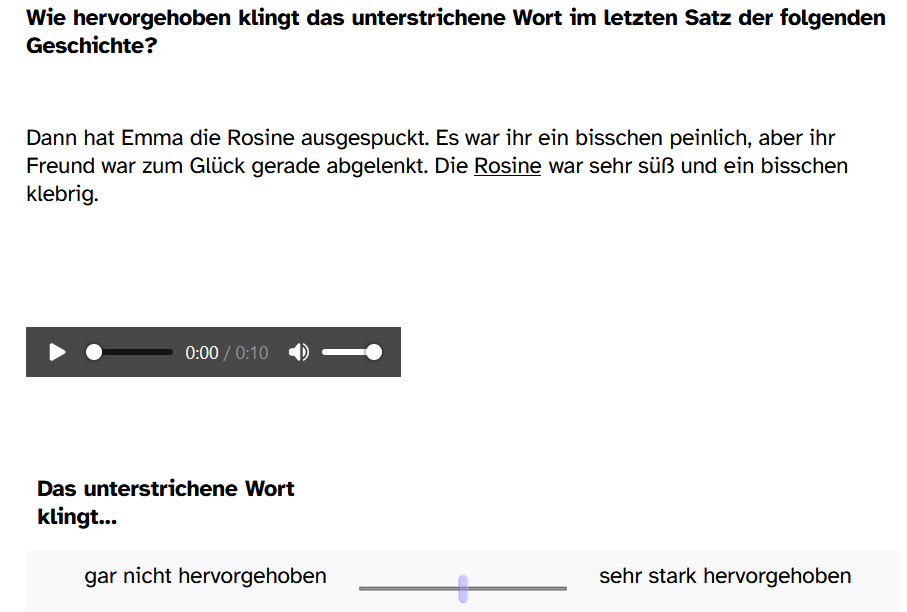
\includegraphics[width=\textwidth]{S3_soscisurvey}
	\caption{Example screen of the prominence rating task implemented in SoSci Survey.}
	\label{fig:S3_soscisurvey}
\end{figure}

Excerpts were sampled from eight different coherent stories, namely the stories recorded in the production study presented in Chapter \ref{ch:Production II}. We selected productions from eight different speakers (three male, five female). Target words were always nouns and appeared in the last sentence of the excerpt but differed in whether they occurred in medial or initial position, as an object or subject, as lexically new or given (i.e., previously mentioned in the same excerpt) and as referentially new or given (i.e., referring to a previously introduced entity in the discourse, see also Table \ref{table:summary_manipulations} in Chapter \ref{ch:Production II}). To ensure that sufficient context would be available to listeners to correctly interpret the lexical and referential information status of the target word, each excerpt consisted of the utterances up until and including the previous mention of the same word (see Figure \ref{fig:S3_soscisurvey} for an example). In the case of the lexically new target words (Target 1), we presented the excerpt from the beginning of the story, which did not include another mention of the same word. 

In addition, target words differed in their prosodic realization, representing a wide range of accent types in prenuclear and nuclear position as well as deaccentuation. We also measured several continuous phonetic parameters in the target words, i.e., the same parameters analyzed in the production experiments presented in Chapters \ref{ch:Production I} and \ref{ch:Production II}: F0 at the Center of Mass (F0 at CoM), Delta F0, Center of Gravity (CoG), synchrony, word and syllable duration, intensity, and periodic energy mass. Table \ref{table:s3_stimuli} summarizes the distributions of the stimuli in terms of accent status and accent type. The feature distributions of the stimuli roughly reflect the distributions observed in the production experiment presented in Chapter \ref{ch:Production II}. The loudness of the recordings was normalized to the same target level before they were entered into the experiment. The stimuli were presented in pseudo-randomized order, ensuring that Target 1 of a story always occurred before the remaining target words, so that the item was truly lexically new to the participants.

\begin{table}[]
\begin{tabular}{llllll}
\lsptoprule
Accent status & Target1 & Target2 & Target3 & Target4 & Target5 \\
\midrule
\multirow{7}{*}{Nuclear}    & 2 L+H*           & 1 L+H*           & 2 L+H*           & 1 L+H*           & 2 L+H*           \\
                            &                  &                  & 2 L*+H           &                  & 2 L*+H           \\
                            & 2 H*             & 1 H*             &                  & 1 H*             &                  \\
                            & 2 H+!H*          & 1 H+!H*          &                  & 1 H+!H*          &                  \\
                            & 1 H+L*           & 1 H+L*           &                  & 1 H+L*           &                  \\
                            & 1 !H*            &                  &                  &                  &                  \\
                            &                  &                  &                  & 1 L*             &                  \\
                            \midrule
\multirow{6}{*}{Prenuclear} &                  & 1 L+H*           & 2 L+H*           & 1 L+H*           & 2 L+H*           \\
                            &                  & 1 L*+H           & 2 L*+H           & 1 L*+H           & 2 L*+H           \\
                            &                  & 1 H*             &                  &                  &                  \\
                            &                  & 1 H+L*           &                  &                  &                  \\
                            &                  & 1 !H*            &                  & 1 !H*            &                  \\
                            &                  & 1 L*             &                  & 1 L*             &                  \\
                            \midrule
Deaccented                  &                  & 2                &                  & 2                &                  \\
\midrule
Total number                       & 8                & 12               & 8                & 11               & 8                \\
\lspbottomrule
\end{tabular}
\caption{Distribution of selected stimuli by target word position, accent status, and accent type.}
\label{table:s3_stimuli}
\end{table}

Responses were collected from 65 monolingual native speakers of German (25 female, 39 male, 1 non-binary) between the ages of 18 and 71 years (mean = 32, SD = 9.6). To the best of our knowledge, none of the participants had taken part in either of the two production studies. Each participant contributed 47 prominence ratings for a total of 3,055 data points. Most participants (n = 55) were from Germany, especially North Rhine-Westphalia, Baden-Wuerttemberg, and Lower Saxony, and ten participants were from Austria. The majority of participants (n = 62) reported no prior experience with speech analysis, three participants had basic experience, and no participant reported any hearing impairment. In addition, we collected information on participants' communicative skill using the same questionnaire as in the study presented in Chapter \ref{ch:Production II} (see Section \ref{sec:Production2 methods} and Appendix \ref{Appendix B} for details), i.e., a subset of the Autism Spectrum Quotient \citep{baron-cohenAutismSpectrumQuotientAQ2006}. Communicative scores in our participants ranged from 1 to 10 (possible values: 0-10, where 0 indicates low and 10 high communicative skill), with a mean of 6.4 (SD = 2.0). Participants were recruited via Prolific (\url{https://www.prolific.co/}) and were paid \pounds 5 for the completion of the experiment. 


\subsection{Statistical analysis}

Statistical analyses were conducted in R \citep{rcoreteamLanguageEnvironmentStatistical2022}. For data wrangling and visualization, we used the \pkg{tidyverse} package \citep{wickhamWelcomeTidyverse2019} and \pkg{cowplot} \citep{wilkeCowplotStreamlinedPlot2020} for arranging multiple plots into one. We ran Bayesian regression models using the \pkg{brms} package \citep{burknerBrmsPackageBayesian2017} as an interface to the Stan modeling language \citep{carpenterStanProbabilisticProgramming2017}. To extract posterior estimates from the models, we used the \pkg{tidybayes} package \citep{kayTidybayesTidyData2023}. The random forest analyses were conducted using the \pkg{party} package \citep{hothornUnbiasedRecursivePartitioning2006}. For the cluster analysis, we made use of the \pkg{cluster} package \citep{maechlerClusterClusterAnalysis2022} and \pkg{ggdendro} \citep{devriesGgdendroCreateDendrograms2024} to create the dendrogram.
Data and scripts are available online (\url{https://osf.io/m5xwe/}).

We used zero-one-inflated beta (zoib) regression models, which are appropriate for data generated using visual analogue scales, where values are bounded between zero and one and values at these two end points tend to be relatively frequent, i.e., ``inflated" \citep{liuZoibPackageBayesian2015, vuorreHowAnalyzeVisual2019}. We ran one model per prominence-cueing parameter (i.e., the continuous and categorical prosodic variables and the syntactic and semantic-pragmatic variables) for a total of 14 models, with prominence rating as the dependent variable in each model. We included the prominence-cueing parameter and communicative score as well as their interaction as predictors, random intercepts for listener, word, and speaker, and by-listener random slopes for the prominence-cueing parameter. Zoib models estimate multiple sets of parameters to capture the distributions of ones and zeros as well as the distribution of any values between one and zero, i.e., the beta regression. However, since only 4.6\% of the data are zeros and 3.2\% are ones, we will focus on the results of the beta regression and disregard the parameters capturing zero-one inflation.

The communicative score variable was centered before being entered into the models so that the model parameters are interpretable with regard to the samples' mean. Prominence ratings were scaled within each listener so that the lowest rating for each individual corresponds to 0 and the highest rating to 1. The continuous prosodic parameters were z-scored to make the model estimates comparable across different measuring units (e.g., semitones or decibels). Finally, we collapsed the annotated GToBI accent types into five categories to simplify the corresponding model and make its interpretation more feasible: rising (L+H* and L*+H), high (H* and !H*), falling (H+L* and H+!H*), low (L*), and deaccented.

Models ran for 4,000 iterations on four chains with a warm-up of 2,000 iterations yielding 8,000 posterior samples per model. We specified weakly informative, normally distributed priors with a mean of zero and a standard deviation of one for the regression coefficients and used the default priors supplied by \pkg{brms} for the remaining parameters. Model fits were assessed by ensuring that no model yielded Rhat values larger than one.

As in the previous analyses, we report model results in terms of the regression coefficient $\beta$ and its 90\% credible intervals (CrIs) under the posterior distributions as well as the posterior probability that $\beta$ is larger than zero: Pr($\beta$\textgreater{}0). We consider the effect of a predictor variable to be reliable if the 90\% credible interval (CrI) does not include 0 and the probability that $\beta$ is larger than zero is higher than 0.95 or lower than 0.05.

In order to investigate inter-individual variability in the prominence ratings, we exploit the by-listener random slopes similar to the analyses conducted in Chapters \ref{ch:Production I} and \ref{ch:Production II}. In contrast to the regression models designed for the production studies, the models here all share the same dependent variable (i.e., prominence rating), so that the model estimates including the random slopes are comparable. This allows us to consider categorical and continuous variables together in the same analysis. Since the variables' accent status and accent type are associated with multiple levels and thus multiple random slope estimates, we averaged the random slope values for each of these variables. We ran a cluster analysis on the extracted random slopes following the same procedure as before (see Section \ref{sec: stats study1} for details), which results in a grouping of listeners which are maximally similar within and dissimilar across clusters.

To establish rankings of all variables in terms of their importance for the prominence ratings, we trained random forest models \citep{breimanRandomForests2001}. Random forests have been argued to be particularly suitable for the analysis of multiple predictors, which are potentially collinear and may interact with each other \citep[e.g.,][]{stroblIntroductionRecursivePartitioning2009}. We entered all 14 prosodic and non-prosodic variables as predictors of prominence ratings as the outcome variable into the same model. Models were trained on 70\% of the data and the remaining 30\% of data were used to validate the model by ensuring that the model predictions were correlated with the unseen data. 

\section{Results} \label{sec:s3_results}

\subsection{Overall results}

In this section, we present the results of the regression models used to probe the effects of the prosodic and non-prosodic parameters on prominence ratings across all listeners. Furthermore, we conduct a random forest analysis to rank the variables in terms of their importance in predicting the prominence ratings. These results will serve as a baseline for the analysis at the individual listener level.

Starting with the categorical prosodic variables, Figure \ref{fig:s3_cat_pros_prmtrs} shows the mean predicted prominence ratings and 90\% CrIs for accent status and accent type. As expected, nuclear accented words are perceived as most prominent and deaccented words as least prominent, with prenuclear accented words in between (see Figure \ref{fig:s3_cat_pros_prmtrs}, left). The estimated difference in prominence ratings between prenuclear and nuclear accented words is reliable according to the respective model ($\beta$ = 0.18, CrI = [0.15; 0.20], Pr($\beta$\textgreater{}0) = 1), as are the differences between deaccented and prenuclear accented ($\beta$ = 0.06, CrI = [0.02; 0.09], Pr($\beta$\textgreater{}0) = 1) and deaccented and nuclear accented words ($\beta$ = 0.23, CrI = [0.20; 0.27], Pr($\beta$\textgreater{}0) = 1). Notably, the difference between prenuclear accented and deaccented target words is much smaller than between prenuclear and nuclear accented target words.

\begin{figure}[b]
		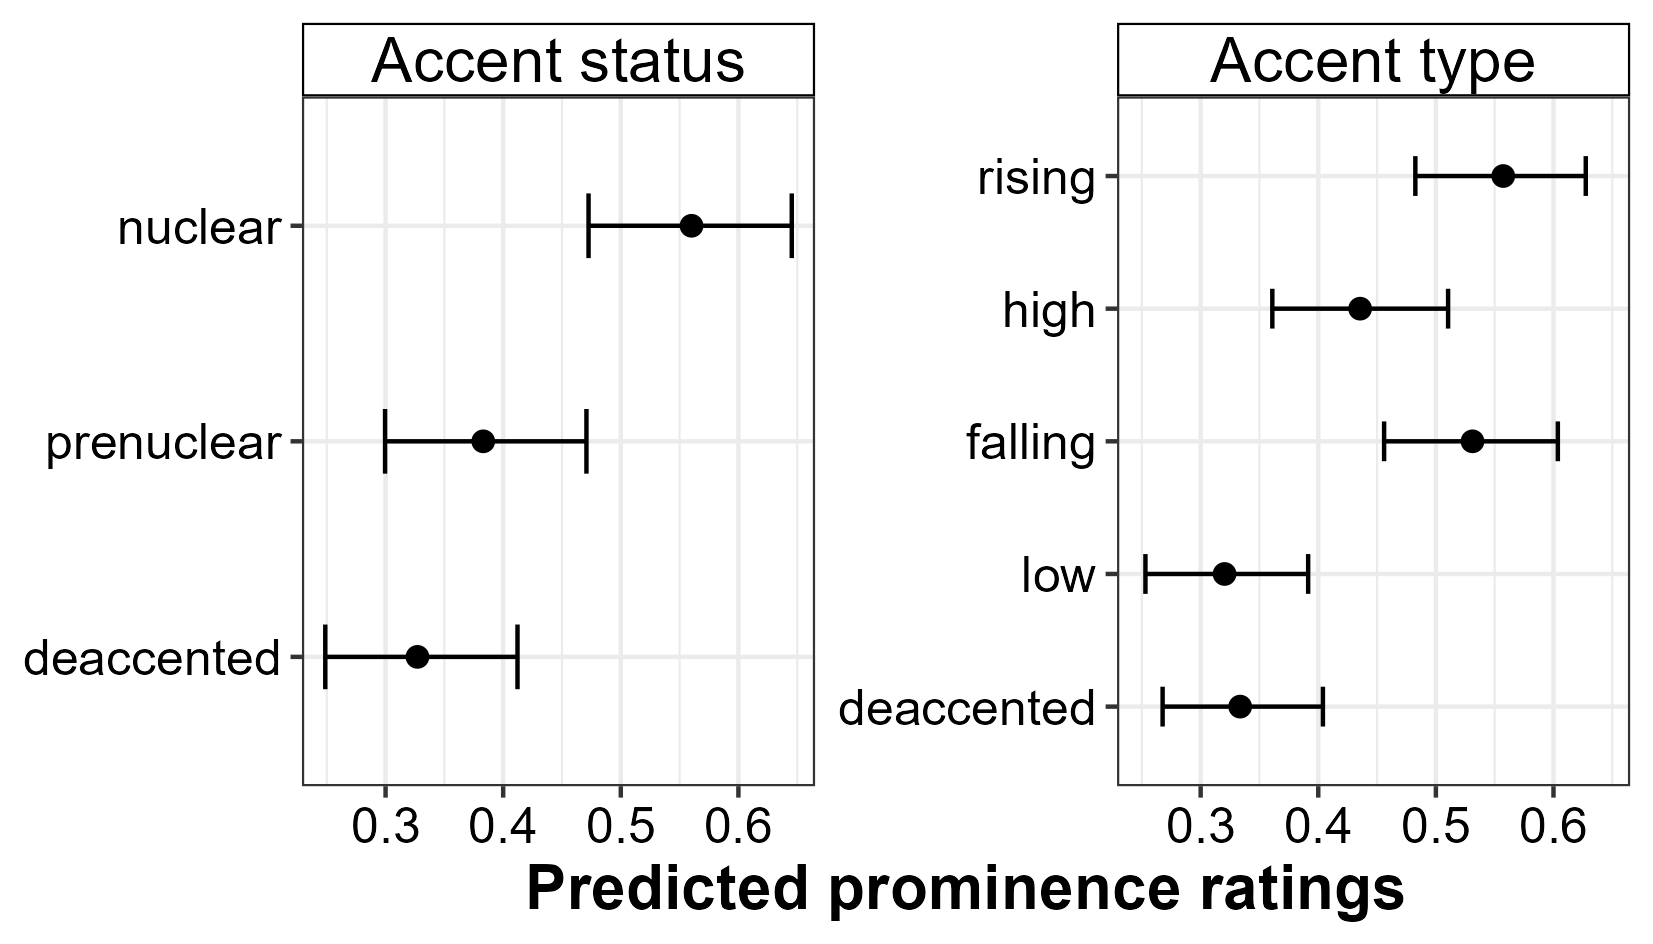
\includegraphics[scale = 0.6]{s3_cat_pros_prmtrs}
	\caption{Mean predicted prominence ratings and 90\% CrIs of the categorical prosodic parameters.}
	\label{fig:s3_cat_pros_prmtrs}
\end{figure}

In terms of accent type, rising accents receive on average the highest prominence ratings, followed by falling and high accents respectively, while low accents and deaccented words are rated least prominent (see Figure \ref{fig:s3_cat_pros_prmtrs}, right). There is a clear advantage for more dynamic accent types, i.e., rising and falling, to be perceived as most prominent, with the direction of pitch movement being of secondary importance. Both rising and falling accents are reliably rated as more prominent than high accents (for rising vs. high: $\beta$ = 0.11, CrI = [0.08; 0.14], Pr($\beta$\textgreater{}0) = 1, for falling vs. high: $\beta$ = 0.09, CrI = [0.06; 0.12], Pr($\beta$\textgreater{}0) = 1). The difference between falling and rising accents is not quite reliable ($\beta$ = 0.02, CrI = [0.0; 0.04], Pr($\beta$\textgreater{}0) = 0.95) but nevertheless provides strong evidence that rising accents are perceived as more prominent than falling ones. Pitch height also plays a role for prominence ratings since high accents are reliably rated as more prominent than low accents ($\beta$ = 0.12, CrI = [0.08; 0.17], Pr($\beta$\textgreater{}0) = 1) or deaccented words ($\beta$ = 0.10, CrI = [0.07; 0.14], Pr($\beta$\textgreater{}0) = 1). Although low accents are on average rated lower in prominence than deaccented words, this difference is not reliable ($\beta$ = -0.01, CrI = [-0.05; 0.03], Pr($\beta$\textgreater{}0) = 0.3).

\begin{figure}[b]
		\includegraphics[scale = 0.6]{S3_cont_prmtrs}
	\caption{Mean posterior estimates and 90\% CrIs of the effects of the continuous prosodic parameters on prominence ratings.}
	\label{fig:S3_cont_prmtrs}
\end{figure}

Additionally, all continuous prosodic variables have a reliable influence on prominence ratings (see Figure \ref{fig:S3_cont_prmtrs} and Appendix \ref{Appendix C} for a plot showing predicted prominence ratings by each continuous prosodic parameter). For most continuous variables, higher values coincide with higher prominence ratings. Longer duration, both of the target word and only the stressed syllable of the target word, reliably predicts higher prominence ratings (for word duration: $\beta$ = 0.17, CrI = [0.15; 0.19], Pr($\beta$\textgreater{}0) = 1, for syllable duration: $\beta$ = 0.15, CrI = [0.13; 0.17], Pr($\beta$\textgreater{}0) = 1). Similarly, words with higher intensity and higher periodic energy mass in the stressed syllable are reliably rated more prominent than words with lower intensity and lower periodic energy mass (for intensity: $\beta$ = 0.08, CrI = [0.06; 0.09], Pr($\beta$\textgreater{}0) = 1, for periodic energy mass: $\beta$ = 0.11, CrI = [0.09; 0.12], Pr($\beta$\textgreater{}0) = 1). As for pitch scaling, both static pitch height measured as F0 at CoM and dynamic pitch change (Delta F0) reliably predict prominence ratings, although the effect of F0 at CoM is much stronger than that of Delta F0 (for F0 at CoM: $\beta$ = 0.12, CrI = [0.11; 0.14], Pr($\beta$\textgreater{}0) = 1, for Delta F0: $\beta$ = 0.01, CrI = [0; 0.02], Pr($\beta$\textgreater{}0) = 0.98). In terms of alignment, words associated with higher synchrony values, which correspond to a more rising F0 within the stressed syllable, are reliably rated more prominent than words with lower synchrony ($\beta$ = 0.03, CrI = [0.02; 0.04], Pr($\beta$\textgreater{}0) = 1). However, unexpectedly, words with an earlier CoG reliably receive higher prominence ratings than words with a later CoG ($\beta$ = -0.06, CrI = [-0.08; -0.05], Pr($\beta$\textgreater{}0) = 0).

\begin{figure}[t]
	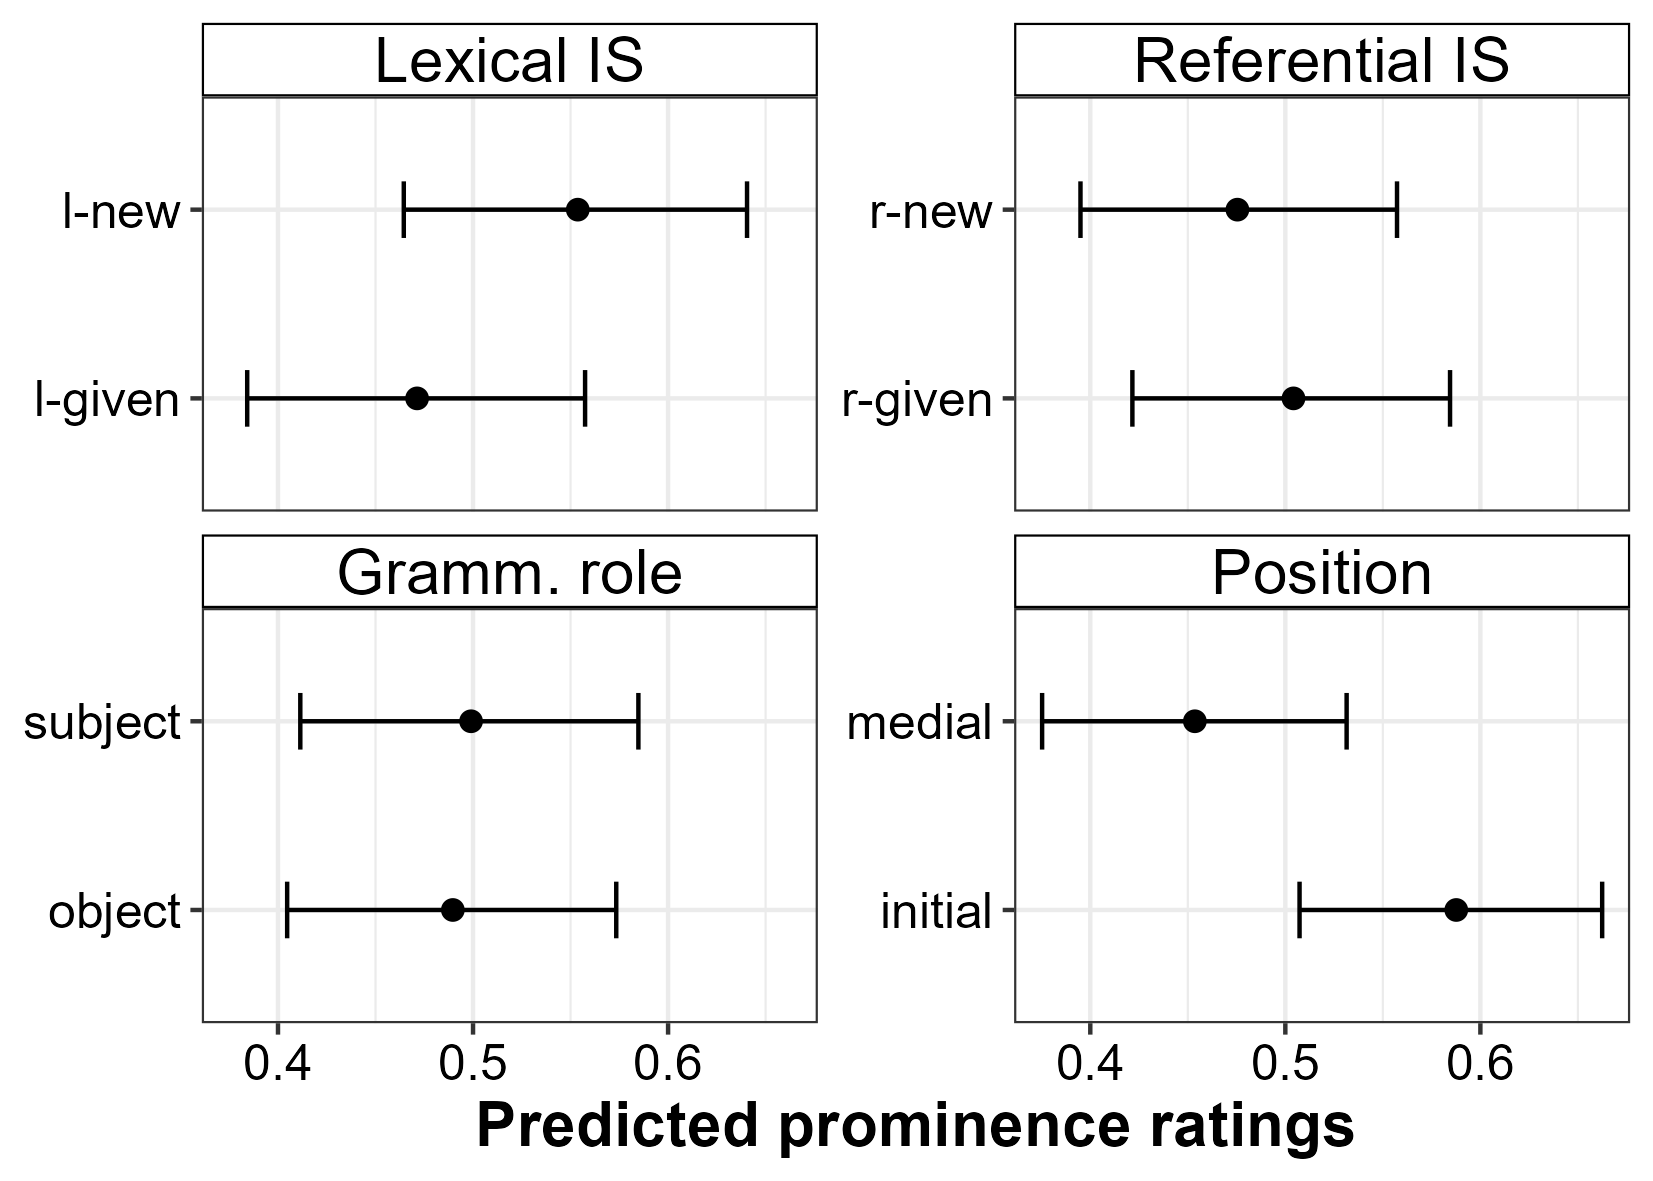
\includegraphics[scale = 0.6]{s3_cat_nonpros_prmtrs}
	\caption{Mean predicted prominence ratings and 90\% CrIs of the non-prosodic parameters.}
	\label{fig:S3_cat_nonpros_prmtrs}
\end{figure}

Finally, we turn to the syntactic and semantic-pragmatic variables. Figure \ref{fig:S3_cat_nonpros_prmtrs} shows the predicted prominence ratings for all four non-prosodic parameters considered here. As expected, lexical newness as opposed to givenness increases prominence ratings across listeners ($\beta$ = 0.08, CrI = [0.06; 0.11], Pr($\beta$\textgreater{}0) = 1). However, the reverse is true for referential information status, with referentially given words reliably rated as more prominent than new ones ($\beta$ = -0.03, CrI = [-0.05; -0.01], Pr($\beta$\textgreater{}0) = 0.01). Grammatical role does not strongly influence prominence ratings ($\beta$ = -0.01, CrI = [-0.03; 0.01], Pr($\beta$\textgreater{}0) = 0.26), but the initial position reliably generates higher prominence ratings than the medial position ($\beta$ = -0.13, CrI = [-0.16; -0.11], Pr($\beta$\textgreater{}0) = 0).

To rank the variables in order of their importance for prominence perception, we turn to random forest analysis \citep[e.g.,][]{breimanRandomForests2001}. The random forest model was first trained on a random subset of 70\% of the data and its predictions were then tested on the remaining 30\% of the data. There is a statistically reliable correlation between the prominence ratings predicted by the random forest model and the actual prominence ratings in the test data ($\beta$ = 0.53, CrI = [0.48; 0.57], Pr($\beta$\textgreater{}0) = 1). The R-squared value we computed (mean R$^2$ = 0.28, CrI = [0.24; 0.31]) indicates that the 14 variables considered in this study account for 28\% of the variance in prominence ratings. 

\begin{figure}
		\includegraphics[scale = 0.7]{S3_random-forest}
	\caption{Variable importance ranking determined by a random forest analysis.}
	\label{fig:S3_random-forest}
\end{figure}

The random forest analysis reveals that accent status is the most important variable in determining prominence ratings across listeners (see Figure \ref{fig:S3_random-forest}). The second discrete prosodic variable, pitch accent type, is also relatively important. Out of the continuous phonetic variables, duration clearly has the largest influence on prominence ratings, especially word duration. CoG and periodic energy mass also rank relatively highly. Delta F0 and intensity are the least important prosodic variables. The syntactic and semantic-pragmatic parameters, by contrast, rank relatively low, the most important of those cues being sentence position, which outranks three of the continuous prosodic cues. Referential information status is slightly more important than lexical information status and grammatical role is the least important variable overall, which is in line with the results of the corresponding regression model.\footnote{Note that the sizes of the parameters' effects on the prominence ratings in the regression models do not necessarily match the results of the random forest analysis. This is due to the fact that some of the parameters are collinear. While the regression models include only one parameter at a time, the random forest analysis takes into account all factors and is thus able to tease apart exactly which parameter contributes most to the prominence ratings and which parameter does not independently contribute. This may explain, for example, why F0 at CoM seems to have a relatively large effect on prominence ratings in the results of the regression models, but ranks below CoG and periodic energy mass in a random forest model that also includes pitch accent type.}

\subsection{Individual strategies}

After reporting on the averaged results across listeners, we turn to the analysis of individual differences (and similarities). Figure \ref{fig:S3_rating_examples} shows exemplary distributions of prominence ratings by four listeners (before scaling). Descriptively, some individuals (e.g., listeners 114 and 150) seem to avoid the middle range of the slider scale, i.e., values around 50, when rating prominence, instead preferring values slightly below or above 50, which leads to bimodal distributions. In the case of listener 114, there seems to be a three-way distinction. This could suggest that prominence is perceived (at least by some individuals) in a more binary or categorical manner, although some gradience in the ratings is also apparent in these listeners. Other listeners (e.g., 151) produce distributions that are closer to normal, which indicates that they treat prominence as more continuous. The inflated use of the end points of the scale (0 and 100), which is typical of scalar rating experiments \citep[e.g.,][]{vuorreHowAnalyzeVisual2019}, is evident in listener 117.

\begin{figure}[b]
	\includegraphics[scale = 0.5]{S3_rating_examples}
	\caption{Prominence ratings by four listeners as examples of differences in the use of visual analogue scales.}
	\label{fig:S3_rating_examples}
\end{figure}

For a systematic approach to individual differences in prominence ratings, we exploit the random by-listener slopes from the regression models presented in the previous section. The random slopes give insight into the extent to which listeners rely on different cues when rating prominence. Running a cluster analysis on the random slopes allows for the identification of potential different listener strategies. The cluster analysis reveals relatively weak evidence for two groups of listeners (average silhouette width: 0.24). Figure \ref{fig:S3_clusters} (left) shows the resulting cluster affiliations in a dendrogram. The majority of listeners (n = 47, 72\% of all listeners) belong to Cluster 1 and Cluster 2 consists of 18 listeners.

\begin{figure}[b]
		\includegraphics[scale = 0.5]{S3_clusters}
	\caption{Results of cluster analysis. Left: Dendrogram showing cluster affiliations of all listeners. Right: Group averages and 90\% CrIs of the posterior estimates for each parameter per cluster.}
	\label{fig:S3_clusters}
\end{figure}

The mean regression coefficients and 90\% CrIs of each variable per cluster are plotted in Figure \ref{fig:S3_clusters} (right). Evidently, the two clusters are very similar in their use of all cues, prosodic and non-prosodic, when rating prominence. Small differences emerge in the extent to which the two clusters rely on certain cues. Listeners in Cluster 2 appear to be more sensitive to accent status and type than those in Cluster 1. Similarly, the prominence ratings of Cluster 2 are also influenced to a stronger degree by synchrony, word and syllable duration, periodic energy mass, and intensity. The remaining continuous prosodic parameters, F0 at CoM, Delta F0, and CoG do not differ much in their effects across clusters, if anything, Cluster 1 relies slightly more on F0 at CoM than Cluster 2. Similar to the trend observed for the prosodic parameters, prominence ratings of Cluster 2 are also more affected by non-prosodic parameters. While the difference across clusters is subtle at best for lexical information status, it is somewhat more pronounced for referential givenness: Both clusters of listeners rate r-given target words more prominent than r-new ones on average, but this effect is stronger for Cluster 2. Similarly, Cluster 2 is more strongly affected by grammatical role and sentence position, although grammatical role does not have a reliable effect on prominence ratings for either cluster and the initial as opposed to the medial position is perceived as more prominent by both clusters.

We trained random forests for each cluster to establish separate variable importance rankings for each group of listeners. These rankings are plotted in Figure \ref{fig:variable_importance_clusters}. The rankings are very similar across clusters, accent status being the most important predictor of prominence ratings in both clusters and intensity and grammatical role the least important ones.  For Cluster 1, word duration is the second most important variable followed by accent type and syllable duration, which corresponds to the ranking observed across all listeners in the overall results. For Cluster 2, accent type is the second most important variable followed by syllable and word duration. The non-prosodic variables rank relatively low for both clusters, sentence position being slightly more important than referential information status for Cluster 2 and the other way around for Cluster 1.

\begin{figure}
		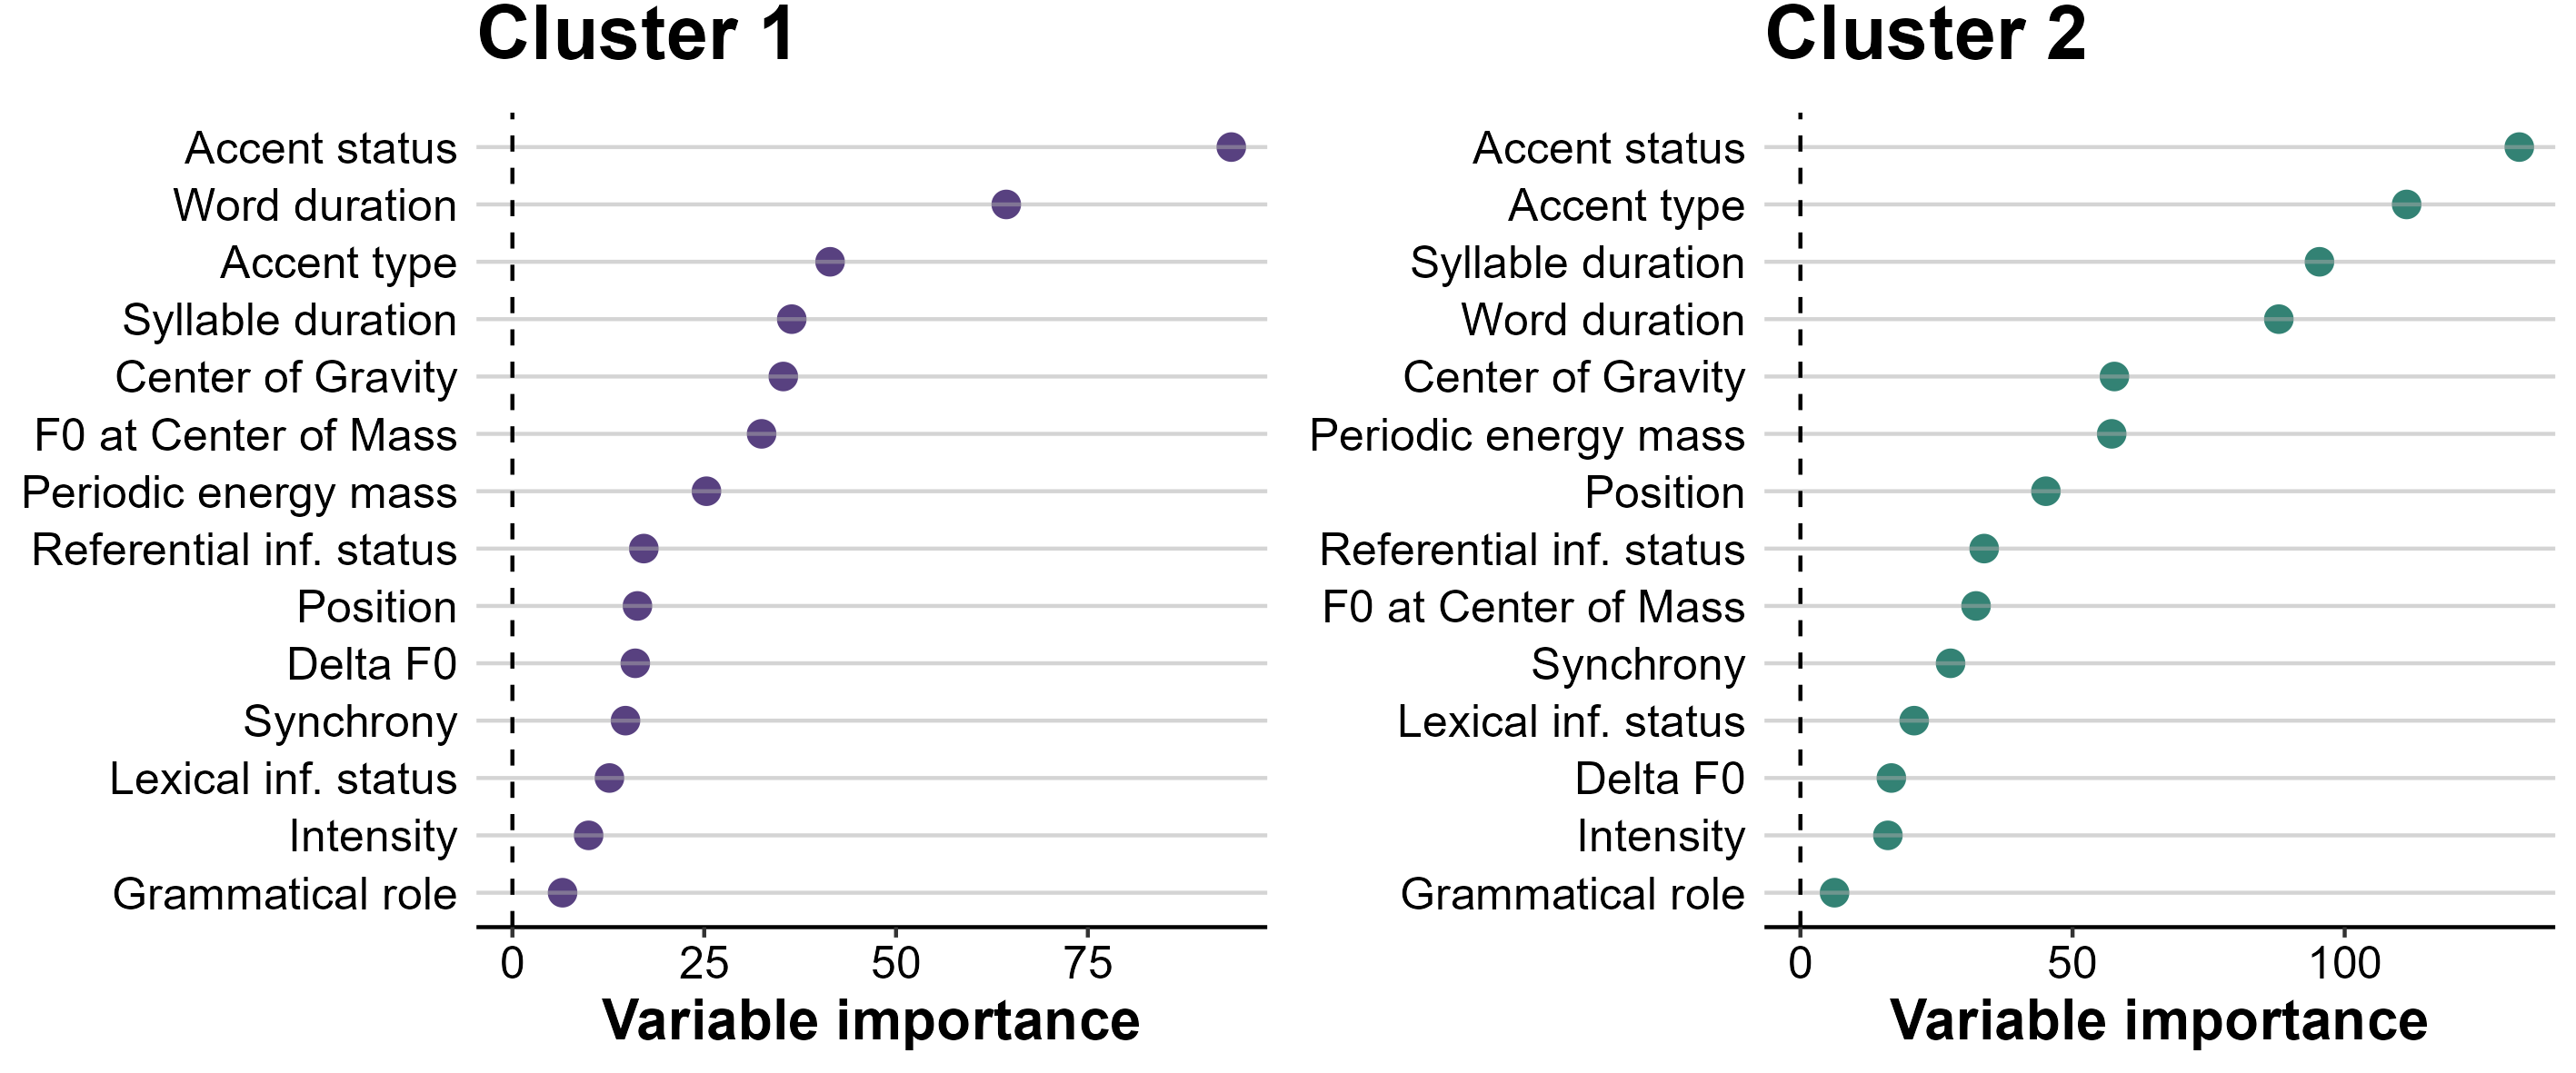
\includegraphics[scale = 0.5]{variable_importance_clusters}
	\caption{Variable importance rankings determined by random forest analyses for each cluster.}
	\label{fig:variable_importance_clusters}
\end{figure}

We again validated the random forest models by testing their predictions on a random subset of 30\% of the data that had been withheld during training. Predicted prominence ratings and actual ratings in the test subset of the data are reliably correlated in both random forests (for Cluster 1: $\beta$ = 0.43, 90\% CrI = [0.37; 0.49], Pr($\beta$\textgreater{}0) = 1, for Cluster 2: $\beta$ = 0.54, 90\% CrI = [0.45; 0.63], Pr($\beta$\textgreater{}0) = 1). We also computed the R-squared values for each cluster as an indication of how much variance is explained by the 14 predictor variables: Cluster 1 is associated with a mean R$^2$ of 0.18 (90\% CrI = [0.14; 0.22]) and Cluster 2 with a mean R$^2$ of 0.29 (90\% CrI = [0.22; 0.36]). The explained variance is thus slightly higher for Cluster 2 than for Cluster 1, in line with the previous observation that this group of listeners is more sensitive to most prominence cues.

As in the second production study presented in Chapter \ref{ch:Production II}, self-assessed communicative scores were collected from all participants. Listeners scored between 1 and 10 points with a mean of 6.4 (SD = 2.0). Generally, listeners with higher communicative scores use higher mean prominence ratings, however, this effect is not reliable for any of the models (e.g., in the accent type model: $\beta$ = 0.01, CrI = [-0.01; 0.02], Pr($\beta$\textgreater{}0) = 0.77). More importantly, we were interested in the interactions between communicative score and the predictor variables, which give insight into the question whether listeners with higher communicative scores are more sensitive to any of the investigated cues in their prominence ratings. Figure \ref{fig:s3_interactions} shows the predicted prominence ratings as a function of the categorical prosodic parameters and communicative score (top) as well as the posterior estimates for the interaction effects of the continuous prosodic cues (bottom left) and the non-prosodic cues (bottom right) with communicative score. 

\begin{figure}
		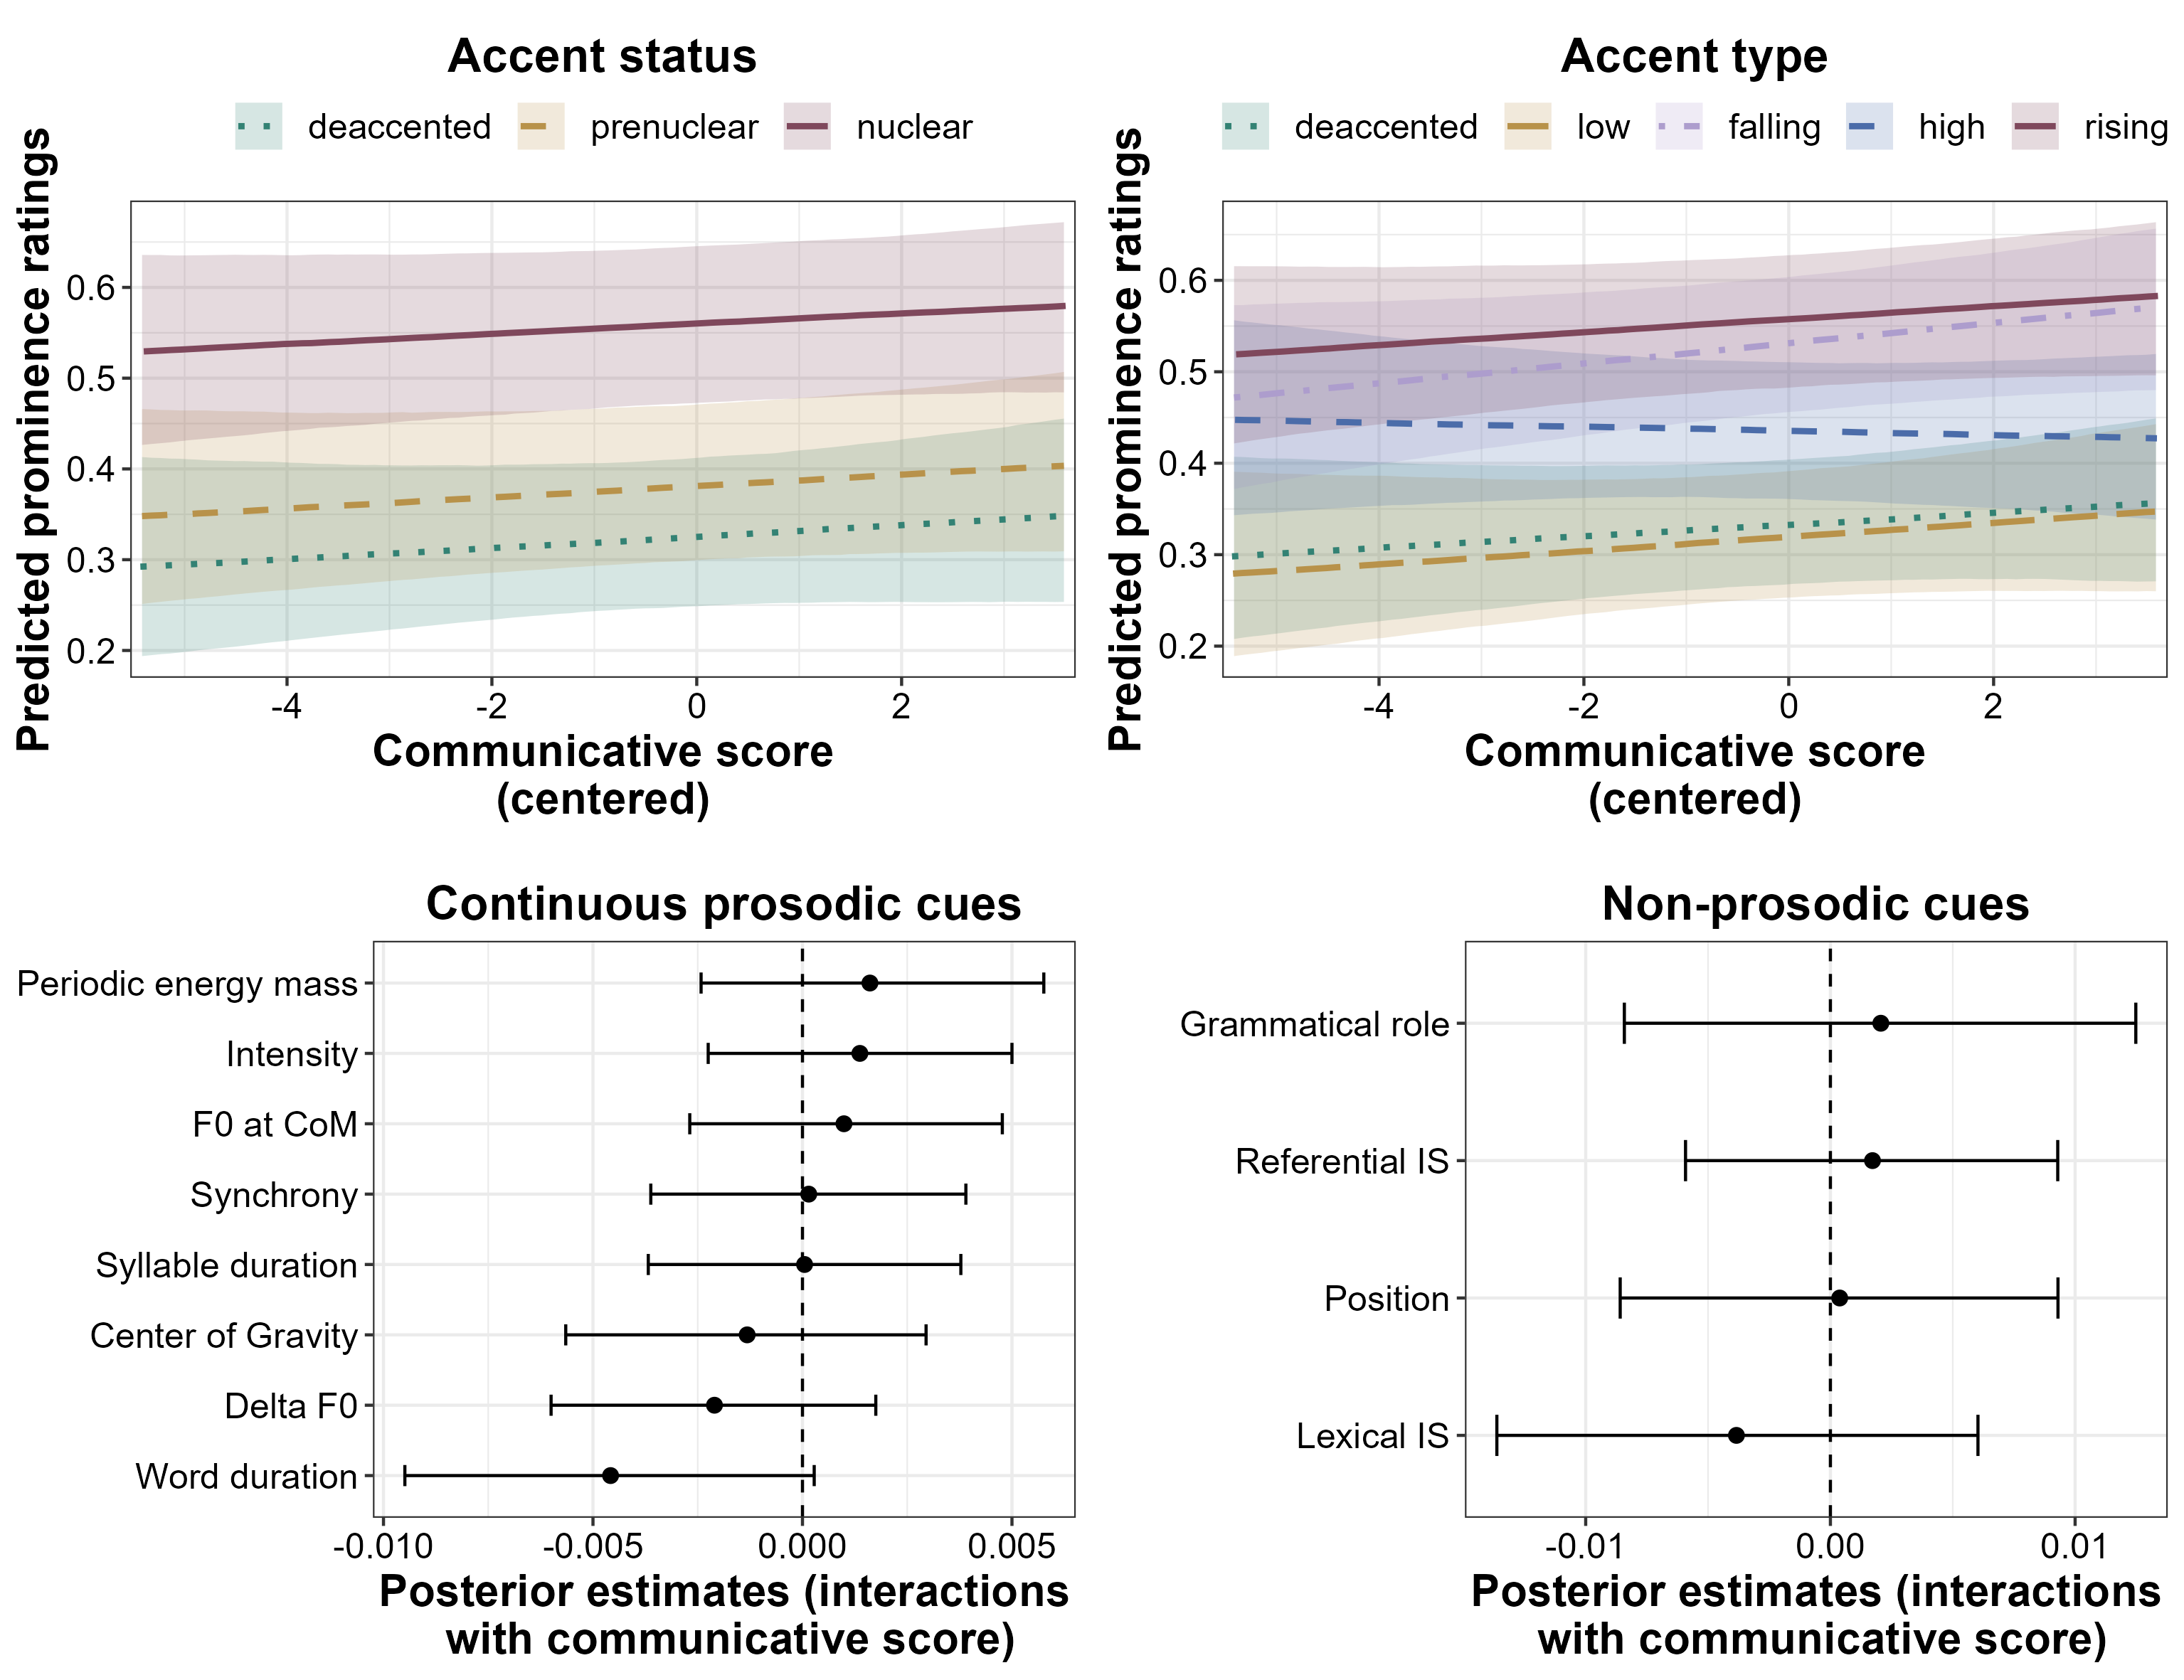
\includegraphics[scale = 0.45]{s3_all_interactions}
	\caption{Interaction effects of the predictor variables and communicative score. Top left: Mean predicted prominence ratings and 90\% CrIs as a function of accent status and communicative score. Top right: Mean predicted prominence ratings and 90\% CrIs as a function of accent type and communicative score. Bottom left: Mean posterior estimates and 90\% CrIs for the interactions of communicative score with the continuous prosodic cues. Bottom right: Mean posterior estimates and 90\% CrIs for the interactions of communicative score with the non-prosodic cues.}
	\label{fig:s3_interactions}
\end{figure}

Since the categorical prosodic cues have multiple levels, we plot the predicted prominence ratings by communicative score for each level (Figure \ref{fig:s3_interactions}, top) and explore them descriptively. The positive main effect of communicative score on prominence ratings is evident from the predominantly positive slopes in the plotted lines. However, for accent status, the three lines for deaccentuation, prenuclear and nuclear accents run in parallel, indicating that there is no interaction between accent status and communicative score. Listeners attend to changes in accent status to the same extent irrespective of their communicative score, only the baseline of prominence ratings is slightly higher for listeners with higher communicative scores. For accent type, we again observe mostly parallel lines with one notable exception: The line associated with the high pitch accent has a slight negative slope, which for listeners with higher communicative scores results in a larger difference in predicted prominence ratings between high and falling/rising accents and a smaller difference between high and low accents/deaccented words. For listeners with lower communicative scores, this effect is reversed: The difference between high and falling/rising accents is smaller for them, while the difference between high and low accents/deaccented words is larger. This may suggest a difference in the perception of accent types with regard to prominence that is modulated by communicative skill. However, note that the credible intervals, which clearly overlap in places, indicate some uncertainty with regard to these observations. Listeners with similar communicative skill are thus not perfectly uniform in their prominence rating behavior. 

In the two bottom plots of Figure \ref{fig:s3_interactions}, posterior estimates indicate how much listeners are influenced by the respective cue in their prominence ratings as a function of communicative score. A mean posterior estimate of 0 indicates that listeners are influenced by a cue to the same extent, irrespective of their communicative score. A positive posterior estimate indicates that listeners with \textit{higher} communicative scores are more strongly influenced by a specific cue in their prominence rating, a negative posterior estimate indicates that listeners with \textit{lower} communicative scores are more strongly influenced by a cue. As is evident from the plots, neither continuous prosodic nor non-prosodic cues reliably interact with communicative score. In fact, many posterior estimates are firmly centered around 0. Out of all these cues, word duration shows the strongest interaction with communicative score, but it is a negative effect: Listeners with lower communicative score are thus more sensitive to differences in word duration when rating prominence. Generally, the results do not provide strong evidence for a consistent effect of communicative score on prominence perception.

Although this is not the primary objective of the present study, a brief note on sociodemographics is in order, since the participants represent a wide range of backgrounds. Table \ref{table:s3_sociodemographics} summarizes the characteristics of listeners in Cluster 1 and 2 in terms of self-reported age, gender, and region of origin.\footnote{The region of origin is based on the federal state in which the participants reported to have grown up in. We classified these states into north and south roughly following the Benrath line.} Listeners in Cluster 1 are younger, more likely female, and from the South than listeners in Cluster 2. However, these differences are relatively small, so that we refrain from drawing any strong conclusions at this point. We will return to this point in the General Discussion in Chapter \ref{ch: general discussion}.

\begin{table}[]
\begin{tabularx}{.9\textwidth}{lYY}
\lsptoprule
                 & Cluster 1 \newline n = 47     & Cluster 2 \newline n = 18     \\ \midrule
Age (median)     & 30                     & 34                     \\
Gender           & 40\% female, 57\% male, 3\% non-binary & 33\% female, 67\% male \\
Region of origin & 28\% north, 72\% south & 39\% north, 61\% south \\
\lspbottomrule
\end{tabularx}
\caption{Sociodemographic characteristics of listeners in the two clusters.}
\label{table:s3_sociodemographics}
\end{table}

\section{Interim discussion} \label{sec:s3_discussion}

In the present study, we confirmed that naive listeners are sensitive to multiple cues in the speech signal when rating prominence on visual analogue scales. Out of 14 potential prosodic and non-prosodic prominence cues, 13 were reliable predictors of prominence. Prosodic cues were especially important in predicting prominence, while syntactic and semantic-pragmatic cues had a much weaker effect on prominence ratings.

The categorical prosodic variables emerged as the strongest cues to perceived prominence, especially accent status but also pitch accent type. This confirms previous findings by \citet{baumannWhatMakesWord2018} and \citet{wagnerExploitingSpeechgestureLink2019} on German as well as \citet{bishopPhonologyPhoneticsSignalextrinsic2020} on American English and provides further independent evidence for the perceptual reality and relevancy of prosodic categories in listeners' processing of prominence. Nuclear accents were clearly perceived as most prominent, while the difference between prenuclear and deaccented words was smaller, underlining the special status of the nuclear accent as a structural cue to prominence \citep[e.g.,][]{buringSemanticsIntonationInformation2007, laddIntonationalPhonology2008}. In terms of pitch accent type, we observed a prevalence of pitch movement over target height: Both rising (L+H*, L*+H) and falling (H+L*, H+!H*) accents were perceived as very prominent, followed by high accents (H*, !H*) and lastly low accents (L*) and deaccented words. This ranking is largely in line with previous observations \citep[e.g.,][]{baumannPerceptualProminencePitch2015, baumannWhatMakesWord2018, bishopPhonologyPhoneticsSignalextrinsic2020}, although some studies have found high accents to be perceived as more prominent than falling accents.

In addition, all continuous variables, capturing aspects of duration, intensity, and fundamental frequency, successfully predicted prominence ratings. Of the continuous parameters, duration was most important, while intensity was the least important predictor of prominence in our study, which is in line with previous studies, such as \citet{fryDurationIntensityPhysical1955, fryExperimentsPerceptionStress1958} and \citet{turkProcessingDurationIntensity1996} but in contrast to \citet{kochanskiLoudnessPredictsProminence2005}. Our study also provides evidence for the validity of the relatively new ProPer measures \citep{albertModelSonorityBased2023} as perceptual correlates of prominence, especially CoG and periodic energy mass. These measures can be derived directly from the signal with no prior annotation, which makes them highly useful for the investigation of larger datasets. With regard to CoG, we expected later alignment to elicit higher ratings, as it has been previously shown that early peaks often correspond to given information, medial peaks to new information and late peaks to unexpected information \citep[e.g.,][]{niebuhrPerzeptionUndKognitive2007}. However, we observed the opposite pattern in that earlier alignment of the CoG elicited higher prominence ratings than later alignment. Interestingly, F0 scaling seemed to add little predictive power independently of pitch accent status and type, which is in line with Fry's (\citeyear[151]{fryExperimentsPerceptionStress1958}) early observation that changes in fundamental frequency ``produce an all-or-none effect" and are interpreted primarily with regard to intonational structure \citep[see also][]{laddProsodicProminenceLanguages2023}.

Of all non-prosodic variables, sentence position was the most important cue to prominence in our listeners, initial target words receiving higher ratings than medial words. Acoustically, the initial position was shown to be produced more prominently than the medial position in Production Study II (see Chapter \ref{ch:Production II}), which partially accounts for the higher ratings. However, the random forest analysis suggests that sentence position also contributed an independent effect. One explanation is that the initial position is less frequent than the medial position in our stimuli and thus more salient through its rarity. In addition, half of the initial stimuli represent a scrambled word order with the grammatical object as initial constituent. In contrast, grammatical role as the second syntactic parameter considered here did not independently contribute to the perception of prominence.

Information status, both lexical and referential, had a relatively small effect on prominence ratings, which could be taken to underline the importance of the prosodic marking of these pragmatic categories. In addition, referential information status behaved opposite to what we expected: Given was perceived as more prominent than new. This could indicate that the short excerpts presented during our task might not have been sufficient for listeners to derive adequate discourse representations or that listeners guided by the task focused more on the prosody of the signal and less on its meaning \citep[e.g.,][]{coleSoundStructureMeaning2019}. Another potential explanation is a mismatch between expectations and prosodic realization: While new referents (at both the lexical and the referential level) would be expected to be produced very prominently by listeners, given referents would be expected to be prosodically attenuated, i.e., deaccented or produced with a prenuclear accent. In the present study, we considered a variety of accent types including nuclear accents on given referents, which are unexpected in this condition. According to \citet{calhounCentralityMetricalStructure2010}, such mismatches in expected and actual prosodic prominence are at the core of prominence perception.

The variables included in the present study as predictors of prominence account for considerably less variability (i.e., 27\%) than previous studies, e.g., by \citet{arnoldUsingGeneralizedAdditive2013}, \citet{baumannWhatMakesWord2018}, and \citet{wagnerExploitingSpeechgestureLink2019}, who accounted for 85\%, 71\%, and 60\% of variability in their respective studies. Some methodological differences to the present study may help explain these discrepancies. For one, \citet{baumannWhatMakesWord2018} and \citet{wagnerExploitingSpeechgestureLink2019} used classic Rapid Prosody Transcription (RPT), where listeners make a binary choice with regard to whether they perceive a word as prominent or not \citep[e.g.,][]{coleSignalbasedExpectationbasedFactors2010}. \citet{arnoldUsingGeneralizedAdditive2013} by contrast obtained prominence ratings on a scale of 0 to 31 from three trained annotators.\footnote{Using prominence scores obtained from trained annotators on visual analogue scales ranging from 0 to 31, \citet{wagnerExploitingSpeechgestureLink2019} were also able to reach 80\% explained variability, similar to \citet{arnoldUsingGeneralizedAdditive2013}.} The use of visual analogue scales, especially by untrained listeners, may introduce more noise than binary RPT ratings. Perhaps more importantly, previous studies included lexical factors, such as part-of-speech and lexical frequency, which were controlled for in our study. Allowing target words to vary in their lexical factors, those studies also included function words, which are generally acoustically not very prominent. As \citet{coleNewMethodsProsodic2016} report, raters are more likely to agree on the absence rather than the presence of prominence, which could have contributed to higher explained variability in those previous studies. In addition, \citet{coleSignalbasedExpectationbasedFactors2010} showed that in American English, lexical frequency is a better predictor of prominence ratings than number of mentions, which is comparable to lexical information status in the present study.

As a further step, we looked at the individual level to reveal potential different strategies in the processing of prominence. However, in contrast to previous studies \citep[e.g.,][]{cangemiListenerSpecificPerceptionSpeakerSpecific2015, bishopIndividualDifferencesTopdown2016, royIndividualDifferencesPatterns2017, baumannWhatMakesWord2018}, we found only subtle individual differences. The main difference between groups of listeners identified via a cluster analysis was the degree of sensitivity to the predictor variables, one group modulating their prominence ratings as a function of these cues a little more than the other group. This was true across prosodic and non-prosodic cues, indicating that the same listeners that were influenced more by prosody also attended more to the syntactic and semantic-pragmatic parameters. This observation is not incompatible with a finding by \citet{orricoInfluenceEmpathyAutisticlike2023}, who report that highly empathetic listeners are more sensitive to the pragmatic distinction of contrastive versus non-contrastive information and highly communicatively skilled individuals are more sensitive to the prosodic contrast of H* versus L+H* accents. Crucially, empathy and communicative skill were correlated in this study, suggesting that the same listeners that were more sensitive to prosody were at the same time more sensitive to pragmatics. Alternatively, higher sensitivity to all types of cues in our study may indicate that some listeners are simply better at performing the prominence rating task, more competent in their use of visual analogue scales or more motivated to perform well.

A plausible explanation for the lack of variability across listeners relates again to the nature of the task: Fairly unambiguously, listeners were asked to rate how highlighted a word sounded, explicitly drawing attention to the acoustic signal. In previous studies \citep[e.g.,][]{baumannWhatMakesWord2018}, the task left more room for interpretation, paraphrasing prominence with terms like ``stressed", ``highlighted" or ``important". That individual differences are minimal in the absence of such alternatives is in line with a finding by \citet{coleSoundStructureMeaning2019} that participants can be guided to focus more on the acoustic signal or the meaning of an utterance by the instructions they receive. Given a straightforward, unambiguous task, which does not lend itself to different interpretations, as is the case in the present study, listeners behave very similarly despite the wide range of cues available to them. In addition, \citet{coleSoundStructureMeaning2019} observed that American English listeners' prominence ratings varied less under different instructions than French or Spanish listeners' ratings. They take this finding to suggest that acoustic prominence and meaning-related factors often coincide in English, which leads to similar prominence ratings under different types of instructions. Assuming a similarly strong link between prosody and meaning in German, this provides further evidence for the concordance of prosodic and non-prosodic cues observed in the present study.

Previous studies \citep[e.g.,][]{bishopPhonologyPhoneticsSignalextrinsic2020, orricoInfluenceEmpathyAutisticlike2023} have noted a correlation between listeners' communicative skill and their ability to perceive prominence distinctions. However, communicative skill did not play an important role in the present study. Nevertheless, some of the tendencies we observed are compatible with the aforementioned previous studies. \citet{bishopIndividualDifferencesTopdown2016} argues that higher communicative skill may specifically be related to a higher sensitivity to pitch but not duration. Our findings support this idea and provide (weak) evidence that listeners with lower communicative skill may in fact be more sensitive to duration. The fact that listeners with lower communicative skill were less sensitive to a distinction between high and rising pitch accents than listeners with higher communicative skill is in line with an observation by \citet{orricoInfluenceEmpathyAutisticlike2023}. \citet{orricoInfluenceEmpathyAutisticlike2023}, who only considered two accent types out of the larger tonal inventory of British English, argue that listeners with lower communicative skill (higher AQ score) mark any accented words as prominent regardless of accent type, which supposedly indicates a poorer integration of context and F0 contour. In the present study, which includes more pitch accent types, we found that listeners with lower communicative skill observed a two-way distinction between rising, high, and falling accents on the one hand and low accents and deaccentuation on the other hand, while listeners with higher communicative skill managed to make a three-way distinction between rising/falling accents, high accents and low accents/deaccentuation.

Most likely, communicative skill (specifically in the way it has been operationalized here) does not fully account for individual variability. A promising avenue for future research is to quantify communicative skill less directly, for example, by measuring performance in tests such as the Reading the Mind in the Eyes test \citep[e.g.,][]{turnbullListenerorientedPhoneticReduction2019}. Another character trait related to communicative skill that may influence the prosody-meaning mapping is empathy \citep[e.g.,][]{esteve-gibertEmpathyInfluencesHow2020, orricoInfluenceEmpathyAutisticlike2023}. \citet{esteve-gibertEmpathyInfluencesHow2020}, for example, found that French listeners with higher empathy scores were more sensitive to intonation as a cue to resolving lexical ambiguities. Additionally, musicality may play a role, especially in pitch perception \citep{schonMusicSpeechMusic2004}. However, future research needs to first and foremost establish the extent of individual variability in prominence perception in the absence of task ambiguities. A comprehensive study should consider prosodic, discourse-related, \textit{and} lexical factors, while controlling for differing task interpretations. Ideally, the task would be communicatively relevant instead of purely metalinguistic to allow participants to form full-fledged discourse representations, which is crucial for the investigation of individual variability in communicative strategies.
